\chapter{Introduction}
\label{sec:intro}

At the heart of programming languages
 lies the question of how to represent and manipulate programs.
Nearly all aspects of programming language work---including
 theorem proving, optimizing compilers, and program synthesis---%
 depend on these fundamental notions,
 since they dictate
 how (and how efficiently!) a tool may
 store and work with programs.
The choice of how to represent and manipulate programs
 largely determines the the efficacy of a tool or technique.

The most common and easily understood
 program representation is the venerable
 \textit{abstract syntax tree} (AST).
An AST is a recursive tree data structure
 where a nodes is an operator and
 some number---potential zero---of children ASTs.
For example, the program $(a * 2) / 2$
 is represented by the AST shown in \autoref{fig:ast1}.
ASTs are the primary data structures used in most programming tools,
 but they are not the only ones.
The most common alternate representation is the \textit{term graph},
 which can be viewed as a variant of ASTs that loosens the tree requirement.
Term graphs can there for capture sharing across common parts of a
 program (also known as a term).
\autoref{fig:ast2} shows a term graph for the program $(a * 2) / 2$.

\begin{figure}
  \subcaptionbox{AST without sharing.\label{fig:ast1}}
    [0.5\linewidth]{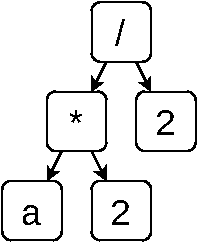
\includegraphics[height=3cm]{ast}}
  \subcaptionbox{Term graph with sharing.\label{fig:ast2}}
    [0.5\linewidth]{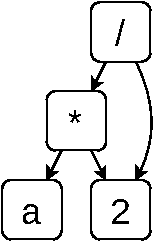
\includegraphics[height=3cm]{ast-sharing}}
  \caption{
    Different representations of the program $(a * 2) / 2$ have
     different characteristics.
    The syntax tree is simpler \subref{fig:ast1},
     but the term graph is smaller since it captures sharing \subref{fig:ast2}.
  }\label{fig:ast}
\end{figure}

\begin{quote}
  \it\Thesisstmt
\end{quote}

\hrule

Equality graphs (\egraphs) were originally developed to
  efficiently represent congruence relations
  in automated theorem provers (ATPs).
At a high level, \egraphs~\cite{nelson, pp-congr}
  extend union-find~\cite{unionfind} to compactly represent
  equivalence classes of expressions while
  maintaining a key invariant:
  the equivalence relation is closed under congruence.\footnote{
    Intuitively, congruence simply means
    that $a \equiv b$ implies $f(a) \equiv f(b)$.}

Over the past decade, several projects have repurposed \egraphs
  to implement state-of-the-art, rewrite-driven
  compiler optimizations and program synthesizers
  using a technique known as \textit{equality saturation}~\cite{
    denali, eqsat, eqsat-llvm, szalinski, yogo-pldi20, spores, herbie}.
Given an input program $p$,
  equality saturation constructs an \egraph $E$ that
  represents a large set of programs equivalent to $p$,
  and then extracts the ``best'' program from $E$.
The \egraph is grown by repeatedly applying
  pattern-based rewrites. % $\ell \to r$.
%Each rewrite $\ell \to r$ includes
%  a pattern $\ell$ to \textit{match} and
%  a pattern $r$ to instantiate and \textit{merge}
%  with the matched subterm.
Critically, these rewrites only add information to the \egraph,
  eliminating the need for careful ordering.
Upon reaching a fixed point (\textit{saturation}),
  $E$ will represent \textit{all equivalent ways} to
  express $p$ with respect to the given rewrites.
After saturation (or timeout),
  a final \textit{extraction} procedure
  analyzes $E$ and selects the
  optimal program according to
  a user-provided cost function.

Ideally, a user could simply provide
  a language grammar and rewrites,
  and equality saturation would produce a effective optimizer.
Two challenges block this ideal.
First, maintaining congruence can become expensive as $E$ grows.
In part, this is because \egraphs from the conventional ATP setting
  remain unspecialized to the distinct \textit{equality saturation workload}.
Second, many applications critically depend on
  \textit{domain-specific analyses}, but
  integrating them requires ad~hoc extensions to the \egraph.
The lack of a general extension mechanism
  has forced researchers to re-implement
  equality saturation from scratch several times~\cite{herbie, eqsat, wu_siga19}.
These challenges limit equality saturation's practicality.

\textit{Equality Saturation Workload. $\,$}
%
ATPs frequently query and modify \egraphs and
  additionally require \textit{backtracking} to
  undo modifications (e.g., in  DPLL(T)~\cite{dpll}).
These requirements force conventional \egraph designs
  to maintain the congruence invariant after every operation.
In contrast,
  the equality saturation workload does not require backtracking and
  can be factored into distinct phases of
  (1) querying the \egraph to simultaneously find all rewrite matches and
  (2) modifying the \egraph to merge in equivalences for all matched terms.

We present a new amortized algorithm
  called \textit{rebuilding} that defers \egraph invariant maintenance
  to equality saturation phase boundaries without compromising soundness.
Empirically, rebuilding provides asymptotic speedups
  over conventional approaches.

\textit{Domain-specific Analyses. $\,$}
%
Equality saturation is primarily driven by syntactic rewriting,
  but many applications require additional interpreted reasoning
  to bring domain knowledge into the \egraph.
Past implementations have resorted to
  ad~hoc \egraph manipulations
  to integrate what would otherwise be
  simple program analyses like constant folding.

To flexibly incorporate such reasoning,
  we introduce a new, general mechanism called \textit{\eclass analyses}.
An \eclass analysis annotates each \eclass
  (an equivalence class of terms)
  with facts drawn from a semilattice domain.
%  resembling an abstract interpretation lifted to \egraphs.
As the \egraph grows,
  facts are introduced, propagated, and joined
  to satisfy the \textit{\eclass analysis invariant},
  which relates analysis facts to the terms represented in the \egraph.
Rewrites cooperate with \eclass analyses by
  depending on analysis facts and
  adding equivalences that in turn
  establish additional facts.
Our case studies and examples
  (Sections \ref{sec:impl} and \ref{sec:case-studies})
  demonstrate \eclass analyses like
  constant folding and free variable analysis
  which required bespoke customization in
  previous equality saturation implementations.

\textit{\Egg. $\,$}
%
We implement rebuilding and \eclass analyses in
  an open-source\footnote{
    \begin{tabular}[t]{ll}
      web: & \url{https://egraphs-good.github.io}\\
      source: & \url{https://github.com/egraphs-good/egg}\\
      documentation: & \url{https://docs.rs/egg}
    \end{tabular}
  }
  library called \egg (\textbf{e}-\textbf{g}raphs \textbf{g}ood).
\Egg specifically targets equality saturation,
  taking advantage of its workload characteristics and
  supporting easy extension mechanisms to
  provide \egraphs specialized for
  program synthesis and optimization.
\Egg also addresses more prosaic challenges,
  e.g., parameterizing over user-defined
  languages, rewrites, and cost functions
  while still providing an optimized implementation.
Our case studies demonstrate how \egg's features
  constitute a general, reusable \egraph library that can
  support equality saturation across diverse domains.

\begin{samepage}
In summary, the contributions of this paper include:
\begin{itemize}
% \item Identifying that equality saturation
%   exposes \egraph to a workload different from
%   theorem provers~\cite{z3} and therefore can benefit from a
%   specialized algorithm for maintaining congruence.
\item Rebuilding (\autoref{sec:rebuilding}),
  a technique that restores key correctness and performance invariants
  only at select points in the equality saturation algorithm.
  Our evaluation demonstrates that rebuilding is faster than
  existing techniques in practice.

\item \Eclass analysis (\autoref{sec:extensions}),
  a technique for integrating domain-specific analyses
  that cannot be expressed as purely syntactic rewrites.
  The \eclass analysis invariant provides the guarantees
  that enable cooperation between rewrites and analyses.


%    a technique for maintaining additional information in \eclasses
%    that enables integrating domain-specific analyses
%    that cannot be expressed as syntactic rewrites.

% \item Identifying the key invariants necessary
%   for a correct, high-performance \egraph library for equality saturation.

\item A fast, extensible implementation of
  \egraphs in a library dubbed \egg (\autoref{sec:impl}).

\item Case studies of real-world, published tools that use \egg
    for deductive synthesis and program optimization across domains such as
    floating point accuracy,
    linear algebra optimization,
    and CAD program synthesis
    (\autoref{sec:case-studies}).
    Where previous implementations existed,
      \egg is orders of magnitude faster and offers more features.
\end{itemize}
\end{samepage}
% The rest of the paper is organized as follows:
% \autoref{sec:background} provides background on term rewriting
%   and defines \egraphs and the invariant, \congrinv.
% It describes the equality saturation workload and how it compares
%   to theorem proving.
% \autoref{sec:rebuild} introduces \egg's novel algorithm
%   for invariant maintenance called \textit{rebuilding}
%   and evaluates it to demonstrate the resulting speedups.
% \autoref{sec:extensions} introduces \eclass analysis and shows
%   how it is used for conditional and dynamic rewrites, and extraction.
% \autoref{sec:impl} discusses the implementation of \egg and
%   presents a partial evaluator for the lambda calculus implemented
%   using \egg.
% \autoref{sec:case-studies} presents three major research projects that
%   have used \egg as their equality saturation engine and benefited
%   in terms of performance and scalability.
% \autoref{sec:related} presents a summary of relevant related work and
% \autoref{sec:conclusion} concludes.


%\Zach{contributions}


%% At a high level, \egraphs~\cite{nelson, pp-congr} store expressions
%%   similarly to the union-find~\cite{unionfind} data structures
%%   often used for representing equivalence relations.
%% The key additional invariant maintained by the e-graph is that its
%%   equivalence relation is closed under congruence.

%  and a performance invariant ($\mathcal{I}_p$) ensuring that
%  equivalent terms are stored without duplication, i.e. equivalent
%  subterms are shared whenever possible.
% \Max{dedup isn't a necessary invariant, it's for perf}

%Equality saturation uses \egraphs to construct $E$,
%  but the resulting workload exhibits distinct phases compared to ATPs and
%  often requires ad~hoc extensions to integrate domain-specific analyses.

% Second, integrating domain-specific analyses
%   requires ad~hoc extensions to the \egraph.
% The lack of a general extension mechanism
%   complicates combining rewrites with analyses.
% These challenges limit equality saturation's practical applicability;
%   researchers have resorted to re-implementing
%   equality saturation from scratch for each new domain.



%%% Local Variables:
%%% TeX-master: "../thesis"
%%% End:
